\documentclass{article}

% Language setting
% Replace `english' with e.g. `spanish' to change the document language
\usepackage[english]{babel}

% Set page size and margins
% Replace 'a4paper' with 'letterpaper' for US standard size
\usepackage[a4paper,top=2cm,bottom=2cm,left=3cm,right=3cm,marginparwidth=1.75cm]{geometry}

% Useful packages
\usepackage{amsmath}
\usepackage{booktabs}
\usepackage{graphicx}
\usepackage[colorlinks=true, allcolors=blue]{hyperref}

\title{Your Paper}
\author{You}

\begin{document}
\maketitle

\begin{abstract}
  Your abstract.
\end{abstract}


\section{Introduction}

The introduction goes here! Simply start writing your document and use the \textit{LaTeX Workshop} extension to build and preview your document.

\section{Some examples to get started}

\subsection{How to create Sections and Subsections}

Simply use the section and subsection commands, as in this example document!

\subsection{How to include Figures}

Use the \textit{includegraphics} command to include it in your document. Use the figure environment and the caption command to add a number and a caption to your figure. See the code for Figure~\ref{fig:cat} in this section for an example.

Note that your figure will automatically be placed in the most appropriate place for it, given the surrounding text and taking into account other figures or tables that may be close by. You can find out more about adding images to your documents in this help article on \href{https://www.overleaf.com/learn/how-to/Including_images_on_Overleaf}{including images}.

\begin{figure}[h]
  \centering
  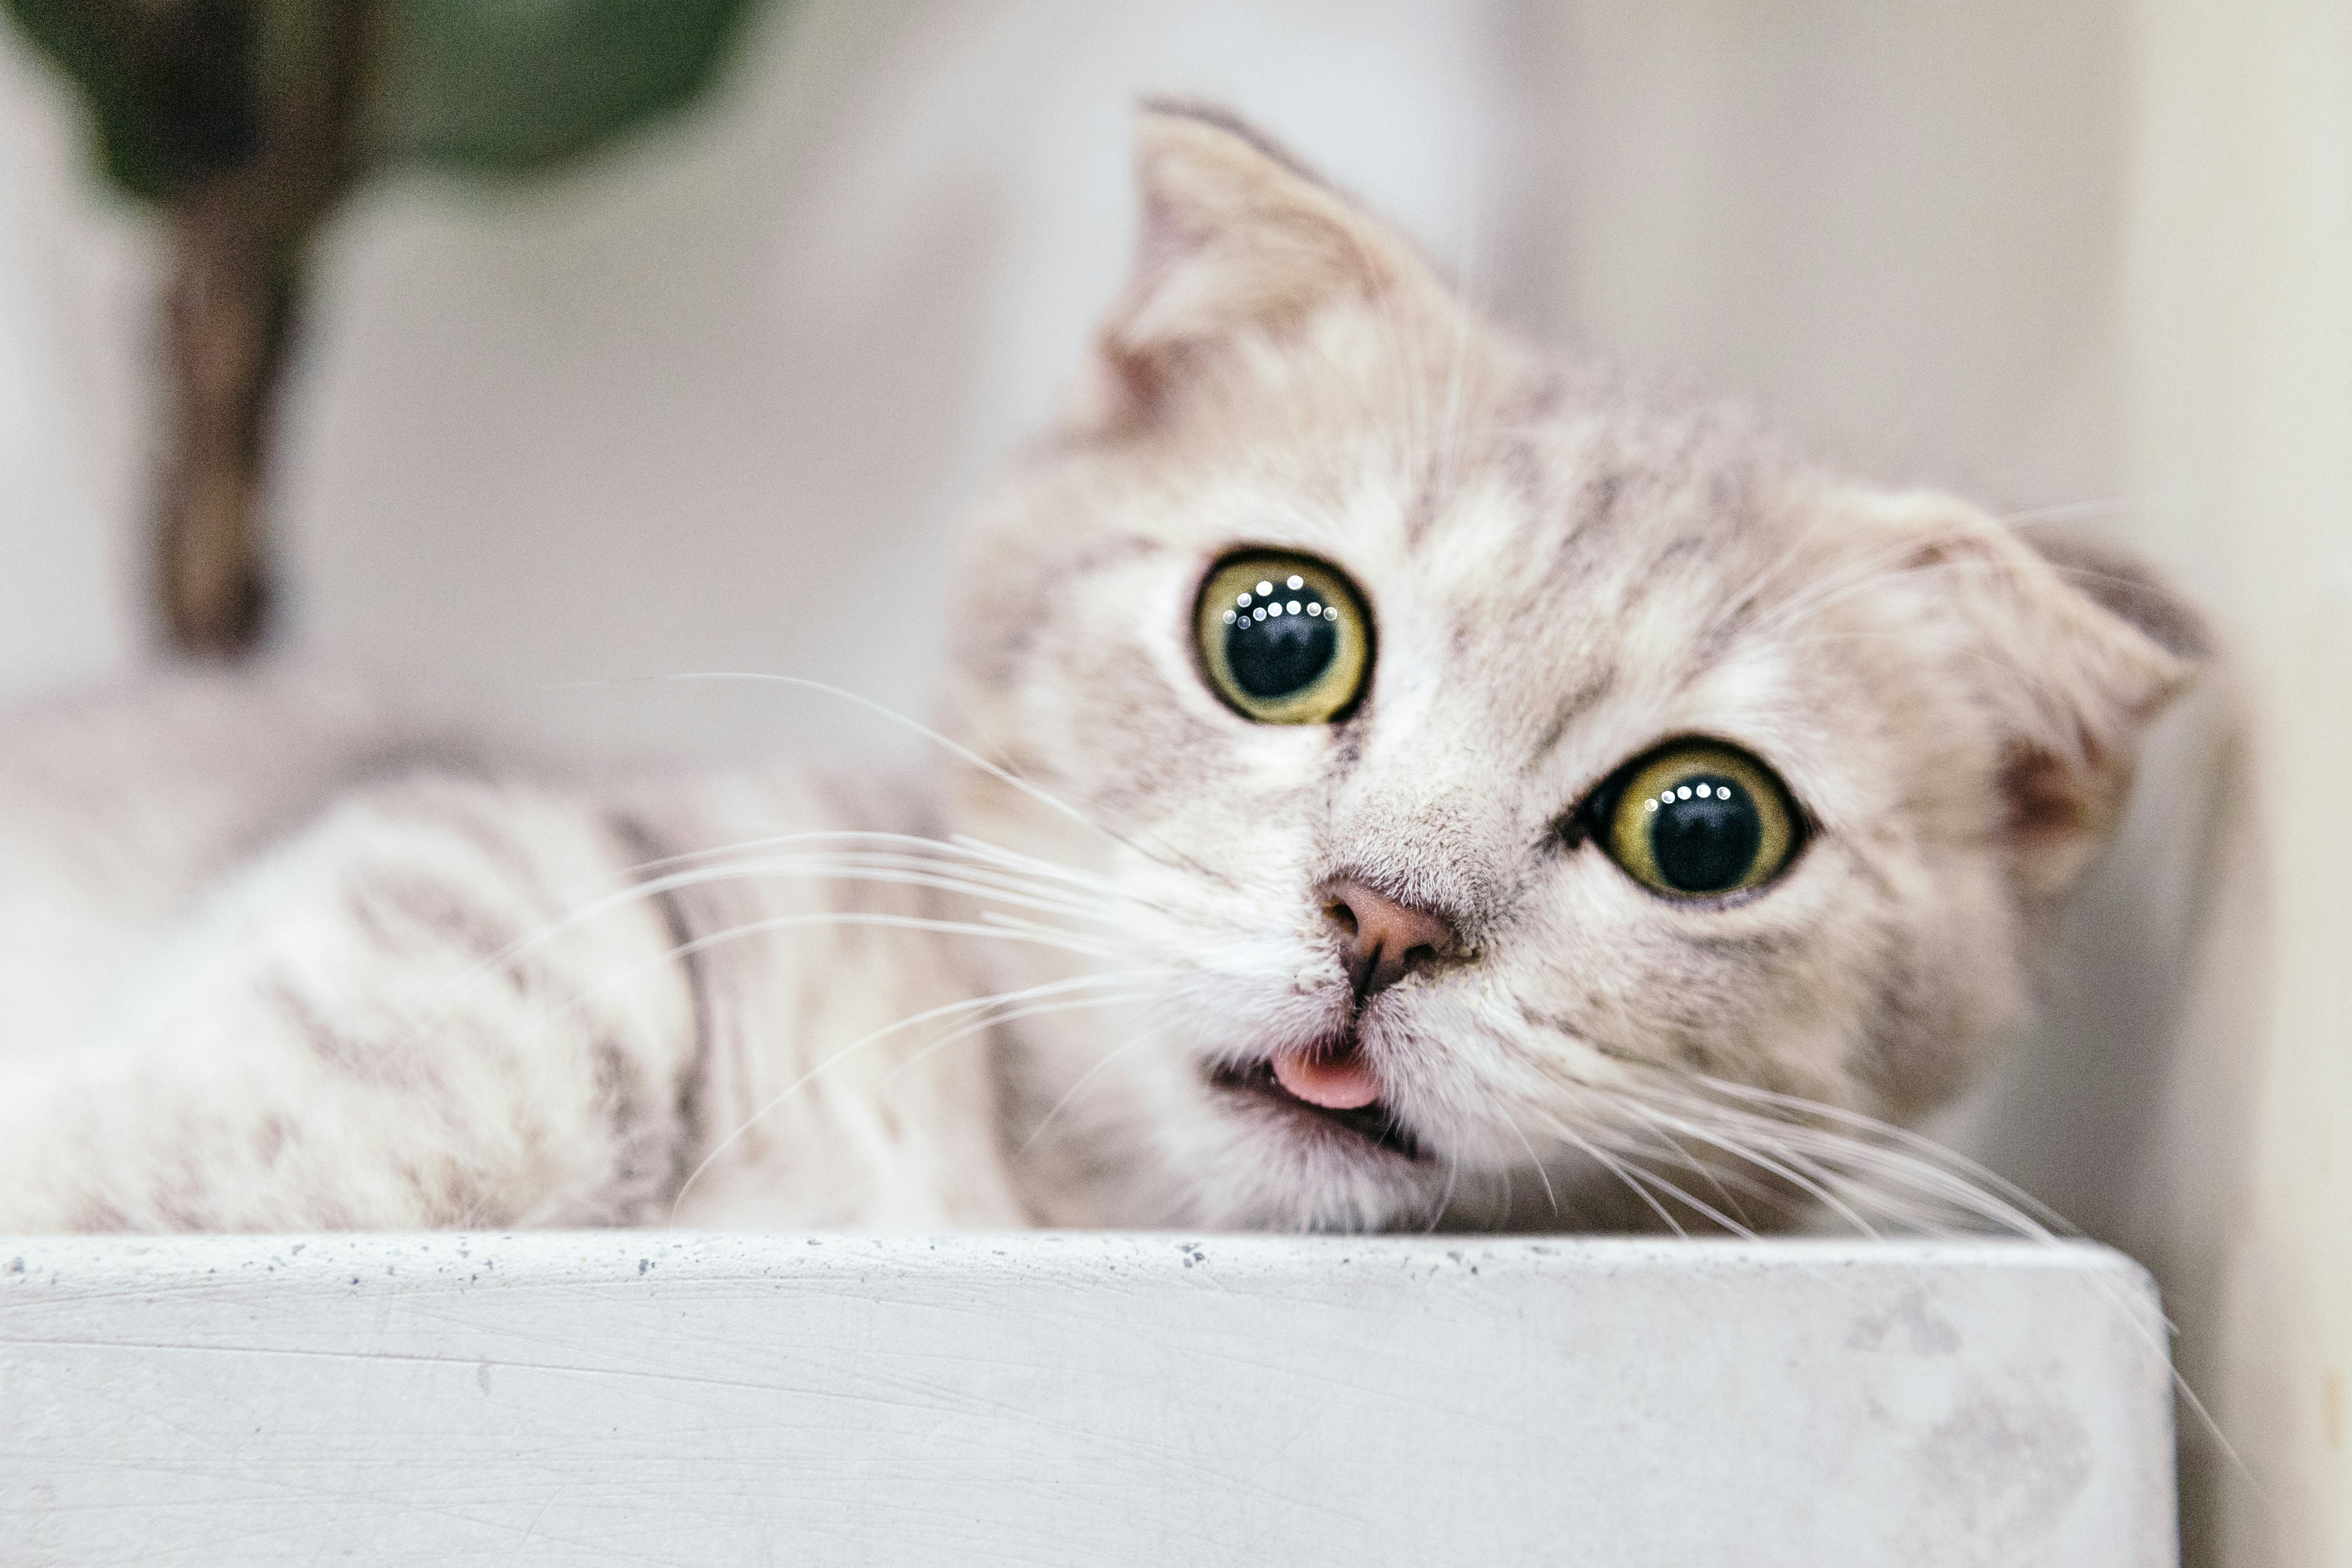
\includegraphics[width=0.6\linewidth]{cat.jpg}
  \caption{\label{fig:cat}Photo by \href{https://unsplash.com/@tranmautritam?utm_content=creditCopyText&utm_medium=referral&utm_source=unsplash}{Tran Mau Tri Tam} on \href{https://unsplash.com/photos/brown-tabby-cat-FbhNdD1ow2g?utm_content=creditCopyText&utm_medium=referral&utm_source=unsplash}{Unsplash}.}
\end{figure}

\subsection{How to add Tables}

Use the table and tabular environments for basic tables {---} see Table~\ref{tab:widgets}, for example. For more information, please see this help article on \href{https://www.overleaf.com/learn/latex/tables}{tables}.

\begin{table}
  \centering
  \begin{tabular}{l c}
    \toprule
    Item    & Quantity \\
    \midrule
    Widgets & 42       \\
    Gadgets & 13       \\
    \bottomrule
  \end{tabular}
  \caption{\label{tab:widgets}An example table.}
\end{table}

\subsection{How to add Lists}

You can make lists with automatic numbering \dots

\begin{enumerate}
  \item Like this,
  \item and like this.
\end{enumerate}
\dots or bullet points \dots
\begin{itemize}
  \item Like this,
  \item and like this.
\end{itemize}

\subsection{How to write Mathematics}

\LaTeX{} is great at typesetting mathematics. Let \(X_1, X_2, \ldots, X_n\) be a sequence of independent and identically distributed random variables with \(\text{E}[X_i] = \mu \) and \(\text{Var}[X_i] = \sigma^2 < \infty \), and let
\[S_n = \frac{X_1 + X_2 + \cdots + X_n}{n}
  = \frac{1}{n}\sum_{i}^{n} X_i\]
denote their mean. Then as \(n\) approaches infinity, the random variables \(\sqrt{n}(S_n - \mu)\) converge in distribution to a normal \(\mathcal{N}(0, \sigma^2)\).

\subsection{How to change the margins and paper size}

Usually the template you're using will have the page margins and paper size set correctly for that use-case. For example, if you're using a journal article template provided by the journal publisher, that template will be formatted according to their requirements. In these cases, it's best not to alter the margins directly.

If however you're using a more general template, such as this one, and would like to alter the margins, a common way to do so is via the geometry package. You can find the geometry package loaded in the preamble at the top of this example file, and if you'd like to learn more about how to adjust the settings, please visit this help article on \href{https://www.overleaf.com/learn/latex/page_size_and_margins}{page size and margins}.

\subsection{How to change the document language and spell check settings}

To configure the document language, simply edit the option provided to the babel package in the preamble at the top of this example project. You may have to install additional language packages, depending on the image you are using for the Dev Container.

The spell check is done using the \href{https://marketplace.visualstudio.com/items?itemName=valentjn.vscode-ltex}{LTex} extension, which is already installed in the Dev Container.

\subsection{How to add Citations and a References List}

You can simply add a \verb|.bib| file containing your BibTeX entries. You can then cite entries from it, like this:~\cite{greenwade93}. Just remember to specify a bibliography style, as well as the filename of the \verb|.bib|. You can find a \href{https://www.overleaf.com/help/97-how-to-include-a-bibliography-using-bibtex}{video tutorial here} to learn more about BibTeX.

\subsection{Good luck!}

Now just open the repository inside the Dev Container and start writing your LaTeX document!

This tutorial is based on the \href{https://www.overleaf.com/latex/templates/example-project/qzykddzqhkwk}{Example Project} template by Overleaf.

\bibliographystyle{alpha}
\bibliography{sample}

\end{document}
